\documentclass{standalone}
\usepackage{fontspec}
\setsansfont{DejaVu Sans}
\usepackage{tikz}
\usetikzlibrary{arrows.meta}
\begin{document}
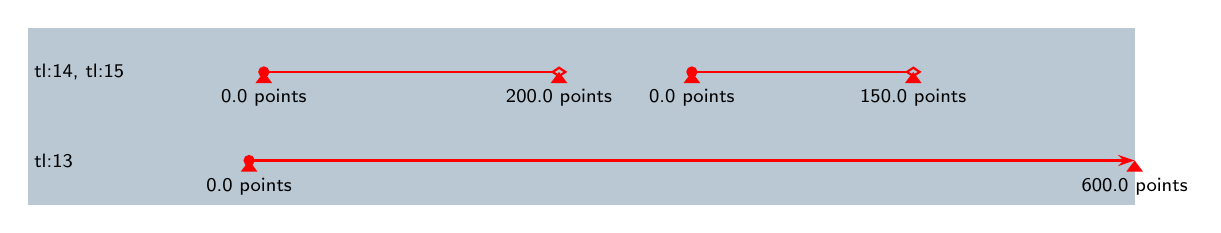
\begin{tikzpicture}[x=1pt,y=1pt,line width=0.8pt,inner sep=2pt,font=\sffamily\fontsize{7}{8.4}\selectfont]
\definecolor{ts000000}{HTML}{000000}
\definecolor{tsBAC8D3}{HTML}{BAC8D3}
\definecolor{tsFF0000}{HTML}{FF0000}
\fill[tsBAC8D3] (0,0) rectangle (400,64);
\draw[tsFF0000,{Circle[length=4pt]}-{Stealth[length=6pt,width=4pt,inset=2pt]},shorten <=-2pt] (80,16) -- (400,16);
\draw[tsFF0000,{Circle[length=4pt]}-{Diamond[open,length=6pt,width=4pt]},shorten <=-2pt,shorten >=-3pt] (85.3333,48) -- (192,48);
\draw[tsFF0000,{Circle[length=4pt]}-{Diamond[open,length=6pt,width=4pt]},shorten <=-2pt,shorten >=-3pt] (240,48) -- (320,48);
\fill[tsFF0000] (80,16) -- (77,12) -- (83,12) -- cycle;
\fill[tsFF0000] (400,16) -- (397,12) -- (403,12) -- cycle;
\fill[tsFF0000] (85.3333,48) -- (82.3333,44) -- (88.3333,44) -- cycle;
\fill[tsFF0000] (192,48) -- (189,44) -- (195,44) -- cycle;
\fill[tsFF0000] (240,48) -- (237,44) -- (243,44) -- cycle;
\fill[tsFF0000] (320,48) -- (317,44) -- (323,44) -- cycle;
\node[anchor=west,text=ts000000] at (0,48) {tl:14, tl:15};
\node[anchor=west,text=ts000000] at (0,16) {tl:13};
\node[anchor=north,text=ts000000] at (80,12) {0.0 points};
\node[anchor=north,text=ts000000] at (400,12) {600.0 points};
\node[anchor=north,text=ts000000] at (85.3333,44) {0.0 points};
\node[anchor=north,text=ts000000] at (192,44) {200.0 points};
\node[anchor=north,text=ts000000] at (240,44) {0.0 points};
\node[anchor=north,text=ts000000] at (320,44) {150.0 points};
\end{tikzpicture}
\end{document}
